\documentclass[]{article}

\usepackage{tikz}
\usetikzlibrary{backgrounds}
\usepackage{graphicx}
\usepackage{amsmath}
\usepackage{amsthm}
\usepackage{amssymb}
\usepackage{url}
\usepackage{multirow}
\usepackage{times}
\usepackage{fullpage}
\usepackage{wrapfig}
\newcommand{\comment}[1]{}

\title{CS685: Group 14 \\
Distributed Code Revision Control System}
\author{
\begin{tabular}{ccc}
Satvik Chauhan & Rahul Ajmera \\
\url{satvikc@iitk.ac.in} & \url{rahulaaj@iitk.ac.in} \\
Dept. of CSE & Dept. of CSE \\
\multicolumn{2}{c}{Indian Institute of Technology, Kanpur}
\end{tabular}
}
\date{	% replace by ``initial'' or ``final'' as appropriate
\today}	% replace by actual date of submission or \today

\begin{document}
\maketitle
\begin{abstract}
A distributed revision control system (DRCS), distributed version control or
decentralized version control system (DVCS) keeps track of software revisions
and allows many developers to work on a given project without necessarily
being connected to a common network \cite{wiki}. Some of the popular
distributed version control systems are Git \cite{git}, Mercurial
\cite{mercurial}, darc \cite{darcs}, GNU Bazaar \cite{bazaar} etc. Distributed Version Control
Systems usually follow peer to peer approach rather than client server. So
instead of a central repository to which each client can synchronize their
changes, each peer has a working copy of the codebase. DVCS usually perform
syncronizations by exchanging patches between peers.

In this project we will be implementing a distributed version control
system with basic features like commit, push patch, pull patch, view history,
merging of code files, reverting changes etc.
\end{abstract}
\begin{wrapfigure}{r}{8cm}
\centering
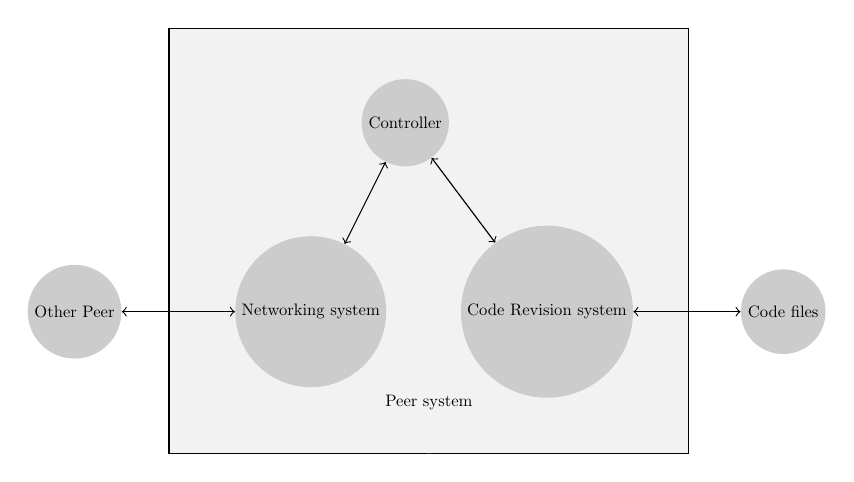
\begin{tikzpicture}[ scale=0.6,transform shape]
\tikzstyle{every node}=[circle,fill=gray!40]
\draw [fill=gray!10] (-3,-3) rectangle (8,6);
\draw (2.5,-3) node [above ,fill=gray!10] {Peer system};
\node (a) at (0,0) {Networking system} ;
\node (b) at (5,0) {Code Revision system};
\node (c) at (2,4) {Controller};
\node (f) at (10,0) {Code files};
\node (u) at (-5,0) {Other Peer};
\draw [<->] (c) -- (a);
\draw [<->] (c) -- (b);
\draw [<->] (u) -- (a);
\draw [<->] (b) -- (f);
\end{tikzpicture}
\end{wrapfigure}
\section{Implementation}
We will take a peer to peer approach for maintaining the code. Every peer will
have its own copy of the codebase and can request other peers to merge their
code with his own codecopy. Unlike CVS, we will not keep a central repository
and every copy of the codebase will be a working copy. The syncronization
between peers will be done by sending patches which will be determined by
using a diff algorithm based on the version of the codes peers haves. We will
keep snapshot for each commit and will follow the git's approach of
compressing the snapshots into blobs \cite{parable}.


\section{Approach}
We will devide the whole project into three subsystems which consists of :

\subsection{Networking}
Networking subsystem implements the underlying communication between the
peers. It consists of
\begin{itemize}
\item Defining the underlying protocol for communication.
\item Connecting to a peer and transferring the patches reported by the
  revision system.
\end{itemize}
\subsection{Code Revision System}
Code Revision system performs all the major tasks of creating blobs, patches and
keeping track of various versions of the code. It consists of
\begin{itemize}
\item Creating blobs and patches based on changes in the files.
\item Determining what patches needs to be send to the peer depending on the
  code version.
\item Merging of the patches to the codebase.
\end{itemize}
\subsection{User Interface/Controller}
This will provide the actual interface which user will be able to use and this
will coordinate the working of the other two components.
It consists of
\begin{itemize}
\item Defining a command line interface for linux machines and if possible a
  gui interface may be considered.
\item Defining the ususal commands like commit, push changes, pull changes
  etc.
\item This will act like a bridge between the networking subsystem and code
  revision system and will combine the features of both to provide an end to
  end distributed version control system.
\end{itemize}

\begin{thebibliography}{99}
\bibitem{wiki}
wikipedia \url{http://en.wikipedia.org/wiki/Distributed_revision_control}
\bibitem{git}
git version control system \url{http://git-scm.com}
\bibitem{mercurial}
Matt Mackall, \emph{Towards a Better SCM: Revlog and Mercurial} .
\bibitem{darcs}
Judah Jacobson, \emph{A formalization of Darcs patch theory using inverse
  semigroups}.
\bibitem{bazaar}
GNU Bazaar, \url{http://wiki.bazaar.canonical.com/}
\bibitem{parable}
Git Parable, \url{http://tom.preston-werner.com/2009/05/19/the-git-parable.html}
\end{thebibliography}

\end{document}